\documentclass[a4paper,12pt]{report}
\usepackage[left=2.0cm, right=2.0cm, top=2.0cm, bottom=2.0cm]{geometry}

\usepackage{graphicx}
\usepackage{setspace}
\usepackage{sectsty}
\usepackage{mathtools}
\usepackage{tkz-euclide}
\usetkzobj{all}
\doublespacing

\author{Matthew Webb}
\title{TorquePaper 2016.2: Steps Required to Achieve Autolock Vision Control}

\newcommand{\tab}{\hspace{20pt}}

\begin{document}
	\maketitle
	\tableofcontents
	
	\chapter{Step 1: Match Turn Angle}
	\section{Camera FOV}
	\tab All cameras have a certain amount of degrees that they can see. The figure below shows how a camera's angle of view translates to an image.
	
	\begin{figure}[h]
		\centering
		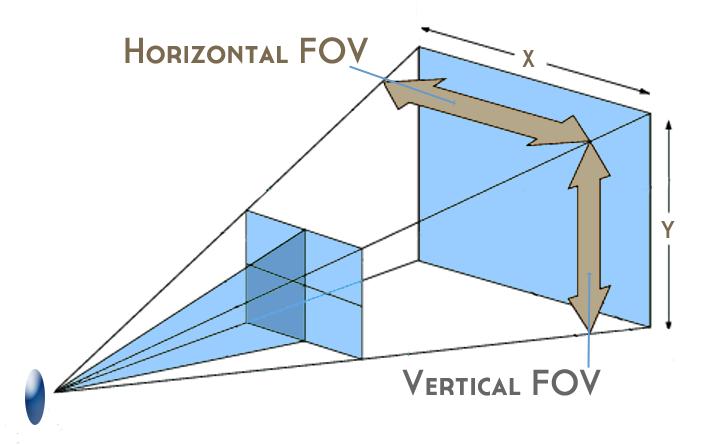
\includegraphics[scale=.3]{camerafov.png}
	\end{figure}
	
	\tab The camera used on Sonic was an Axis Camera M1013 which has an angle of view of 67$^{\circ}$. This means that if the camera faces the front of the robot, the camera will be able to see 33.5$^{\circ}$ left and right.
	\section{Simple Solution}
	\tab OpenCV/GRIP is able to determine the center of the U shape that the reflective tape forms. This means that 
\end{document}